%Created with command:
%"/home/josh/Teaching/trunk/Utilities/makeexam" "Homework 5 - Combinational Design" "Please complete the problems below.  As usual you may work together and use other resources including those in the Internet for reference.  However make sure the work that you submit is yours." "../CombinationalDesign/Assessments/wakerly_6_9.tex" "../Decoders/Assessments/decoder_seven_segment.tex" "../Encoders/Assessments/wakerly_6_51.tex"
\documentclass{article}
\usepackage[T1]{fontenc}
\usepackage{arev}
\usepackage{longtable}
\usepackage[hmargin=2cm,vmargin=2cm]{geometry}
\usepackage{graphicx}
\usepackage{listings}
\setlength{\parindent}{0pt}
\title{Homework 5 - Combinational Design}
\date{}
\begin{document}
\maketitle
Please complete the problems below.  As usual you may work together and use other resources including those in the Internet for reference.  However make sure the work that you submit is yours. (18 points total)
\begin{longtable}[l]{rp{17cm}}
%file: ../CombinationalDesign/Assessments/wakerly_6_9.tex
1.&\begin{minipage}[t]{\linewidth}(2 pt) Do the first part of problem 6.9 in the text (up to, but not including the sentence beginning with the word ``Repeat'').\\ \\

Solution: \\ \\
LOW-to-HIGH: $6 \cdot t_{pLH(Maximum)} = 6 \cdot 15 \textrm{ns} = 90 \textrm{ns}$\\
HIGH-to-LOW $6 \cdot t_{pHL(Maximum)} = 6 \cdot 15 \textrm{ns} = 90 \textrm{ns}$\\
\end{minipage}\\
\medskip
%file: ../Decoders/Assessments/decoder_seven_segment.tex
2.&\begin{minipage}[t]{\linewidth}(10 pt) Design the VHDL architecture for a 3-to-8 decoder with active high inputs and outputs that drives seven segment LED like the one in figure 6-44 of the text.  Assume that a given LED segment is on if its input is high.  The decoder should assume the input is a three bit binary number.  The decimal equivalent of that number will be shown on the LED display.  The decoder should use the following entity:
\begin{verbatim}
entity seven_segment_decoder is
    port (X: in std_logic_vector(2 downto 0);
          F: out std_logic_vector(6 downto 0));
end entity;
\end{verbatim}
I will provide a test bench that you should use to verify your architecture.  The testbench should run using your component without any errors.  Email your .vhd file before the beginning of class on the due date of the assignment.

Solution: \\ \\
\lstset{language=VHDL}
\lstinputlisting{../Decoders/Assessments/seven_segment_decoder.vhd}
\end{minipage}\\
\medskip
%file: ../Encoders/Assessments/wakerly_6_51.tex
3.&\begin{minipage}[t]{\linewidth}(6 pt) Do problem 6.51 in the text.\\ \\

Solution: \\ \\
The inputs are active low, the outputs are active high.\\
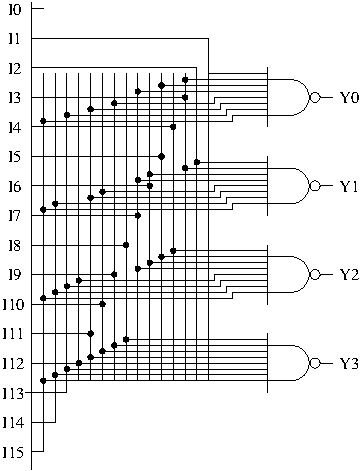
\includegraphics[scale=2.0]{../Encoders/Assessments/wakerly_6_51}
\end{minipage}\\
\medskip
\end{longtable}
\end{document}